\chapter{Simulations Results} 
\section{$Re_{\tau}=180$ simulation} \label{chapter:Re180}

The $Re_{\tau}=180$ simulation has been used to validate our results against the~\cite{kim_moin_moser} ones. \par

The channel length is $4\pi \delta$, while the width is $2 \pi \delta$, with $\delta$ indicating the half channel height. \par
Since our code employ spectral decomposition along the $xy$ plane, we define the streamwise and spanwise periods as $L_{x}= 2\pi /\alpha_{0}$ and $L_{z}=2\pi /\beta_{0}$, with $\alpha_{0}$ and $\beta_{0}$ fundamental wavenumbers. \par
The simulation take place using constant pressure gradient, imposed along $x$ direction, therefore $meanpx=1$.\par
The mesh along $y$ direction is non-uniform, discretized as
\begin{equation*}
y(i)=y_{min}+\frac{1}{2}(y_{max}-y_{min})  \frac{\tanh(a(2i/ny-1))}{\tanh(a)+0.5(y_{max}-y_{min})}
\end{equation*}
with $a=1.6$.\par
The timestep is constant, with $dt=0.0001$ and the simulation time is $T=50$ non dimensional units.
The grid employ 96 modes along $x$ dimension, which, thanks to the Hermitian symmetry, behave as 192 points. The $y$ is discretized using 128 points, while, along the $z$ direction, we have 160 points. The total mesh size reach approximately 2 millions of grid points, decomposed across 512 cores, employed during the simulation. 

The domain and the details about the simulation are summarized in table~\ref{table:180}.\\~\par
\begin{table}[h]
\caption{Simulation data for $Re_{\tau}$=180}
\begin{center}
\begin{tabular}{ccccccccccccc}
\toprule
$L_{x}$ & $L_{z}$ & $\delta$ & $nx$ & $nz$ & $ny$ & $\alpha_{0}$ & $\beta_{0}$ & $\Delta x^{+}$ & $\Delta z^{+}$ & $px$ & $dt$ & $T$\\
$4\pi$ & $2\pi$ & 1 & 192 & 160 & 128 & 0.5 & 1 & 11.8  & 7 & 1 & 0.0001 & 50 \\
\bottomrule
\end{tabular}
\end{center}
\label{table:180}
\end{table}

The bulk mean velocity, defined as 
\begin{equation}
\label{bulk:velocity}
U_{m} = \int_{0}^{1} \bar{u}d \big(\frac{y}{\delta} \big)
\end{equation}

normalized by the wall-shear velocity, is 15.66, which gives the Reynolds number based on the bulk mean velocity and the full channel width, $Re_{b}\approx 5600$. \\~\par
The graphs~\ref{loglaw_180} and~\ref{budget_180} show the behavior of the mean velocity and the roots means squares in the near wall region, with $\bar{u}$ indicating the mean velocity profile. \par
In both figures we reported the \emph{Kim et al.} results, using dotted line, for comparison. \\~\par

\begin{figure}
\begin{center}
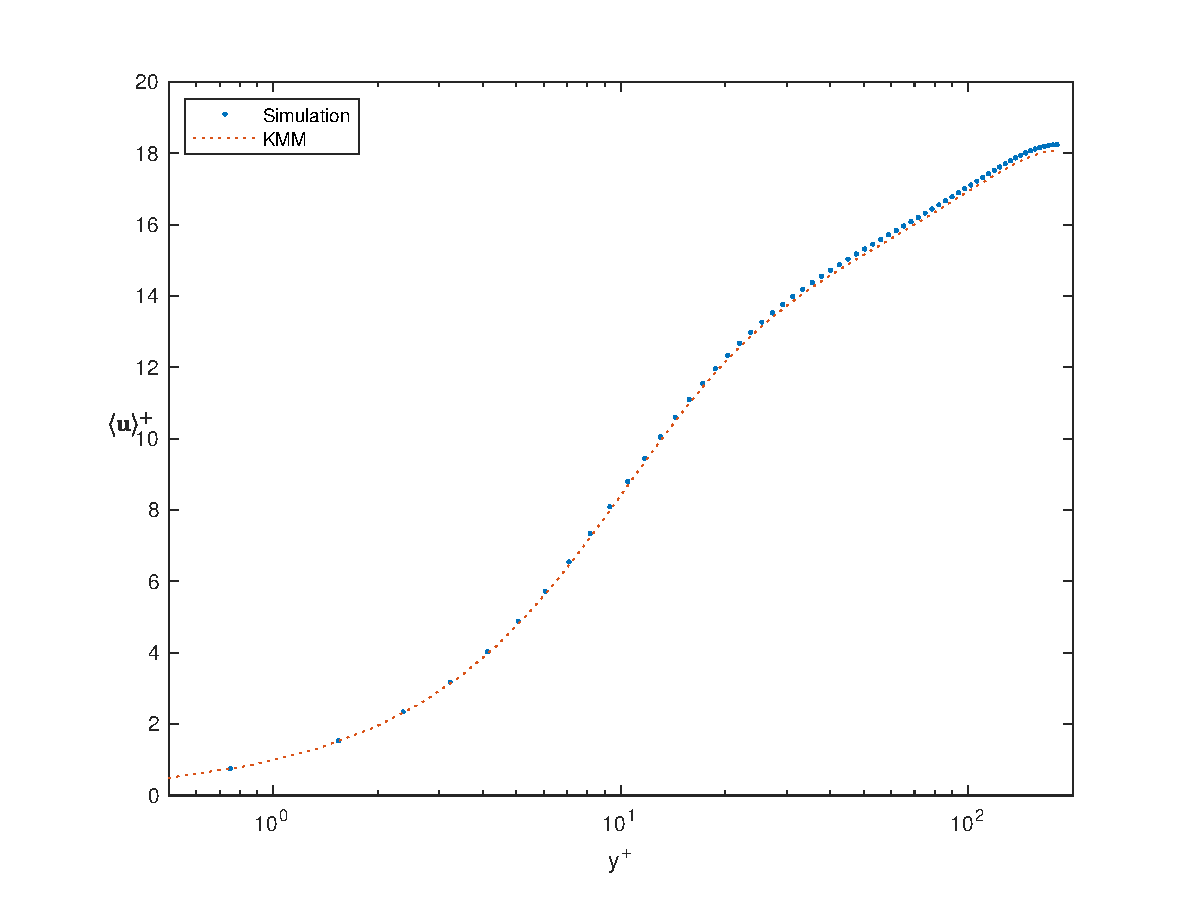
\includegraphics[scale=0.55]{grafici/loglaw_180.eps}
\caption{$\bar{u}^{+}$ in the near wall region for a $Re_{\tau}=180$ simulation}
\label{loglaw_180}
\end{center} 
\end{figure}
\begin{figure}
\begin{center}
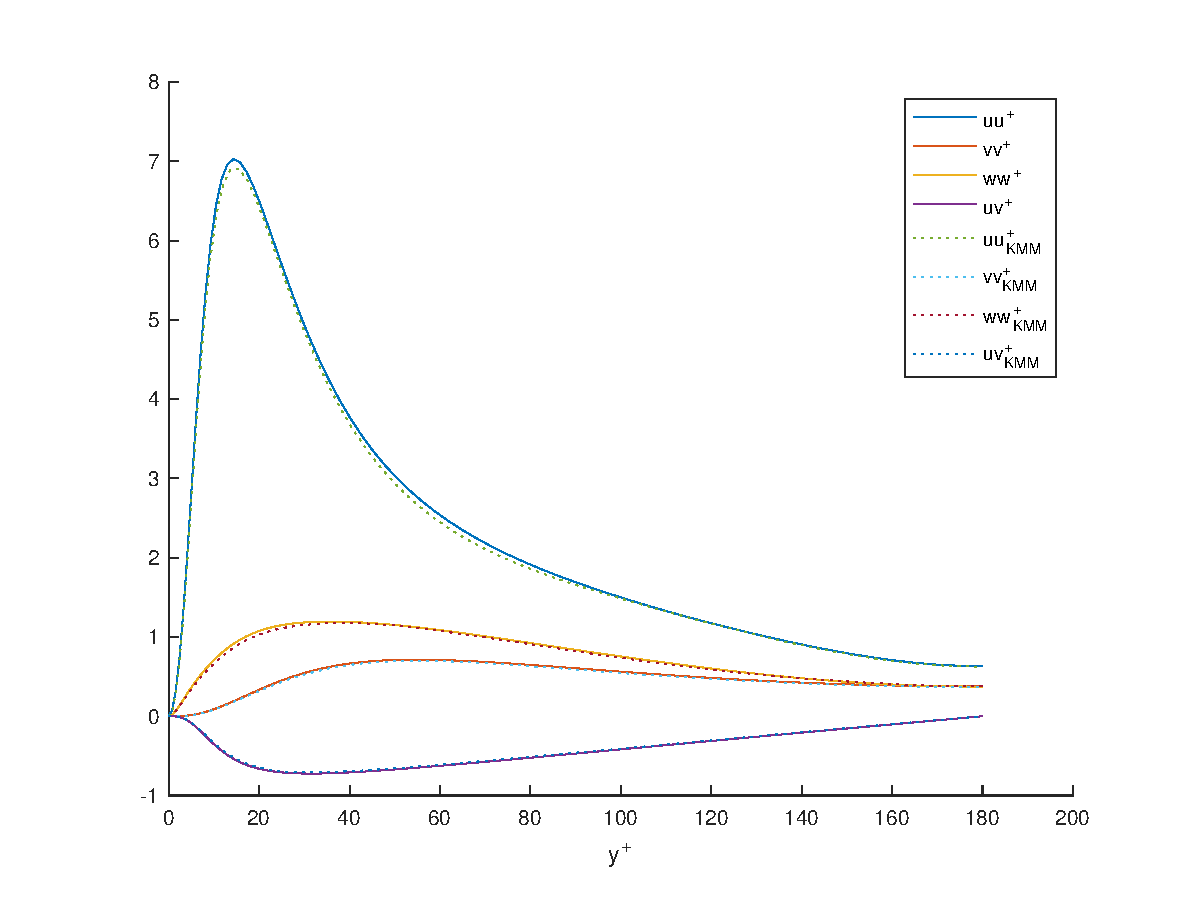
\includegraphics[scale=0.55]{grafici/budget_180.eps}
\caption{\emph{rms} terms for a $Re_{\tau}=180$ simulation}
\label{budget_180}
\end{center} 
\end{figure}


Our statistics have been registered using a simulation time of 50 non dimensional units, sampling data every 0.1 steps.
In total 500 fields have been used to perform the ensemble average. \par

The data fitting is good, despite being perfect. The divergences among our database and the~\cite{kim_moin_moser} ones are possibly due to the fluctuations, rounding errors and differences in averaging times.\\~\par

Nevertheless the results are in agreement with the typical curves behavior, in particular, by looking at the root mean square curves, we can clearly see that $\langle uu\rangle$ and $\langle ww\rangle$ depart from 0 as $y^{2}$, while $\langle uv\rangle$ and $\langle vv\rangle$ increase more slowly, as $y^{3}$ and $y^{4}$, in agreement with~\cite[284]{pope}.
All these information testify that, close to the walls, there is a \emph{two component flow}, with $v=0$ whereas $u$ and $w$ are non-zero. The resulting motion corresponds to flow in planes parallel to the wall. \\~\par

The figure~\ref{loglaw_180} report the $\bar{u}$ behavior near the wall. From 0 up to 5 $y^{+}$ units we can see the typical $\bar{u}=y^{+}$ behavior, which characterize the viscous sublayer. Once $y^{+}>30$ we see the arise of the logarithmic law of the wall, characterized by the equation

\begin{equation*}
\bar{u}^{+} = \frac{1}{\kappa} \ln y^{+} +C^{+},
\end{equation*}


\begin{figure}
\begin{center}
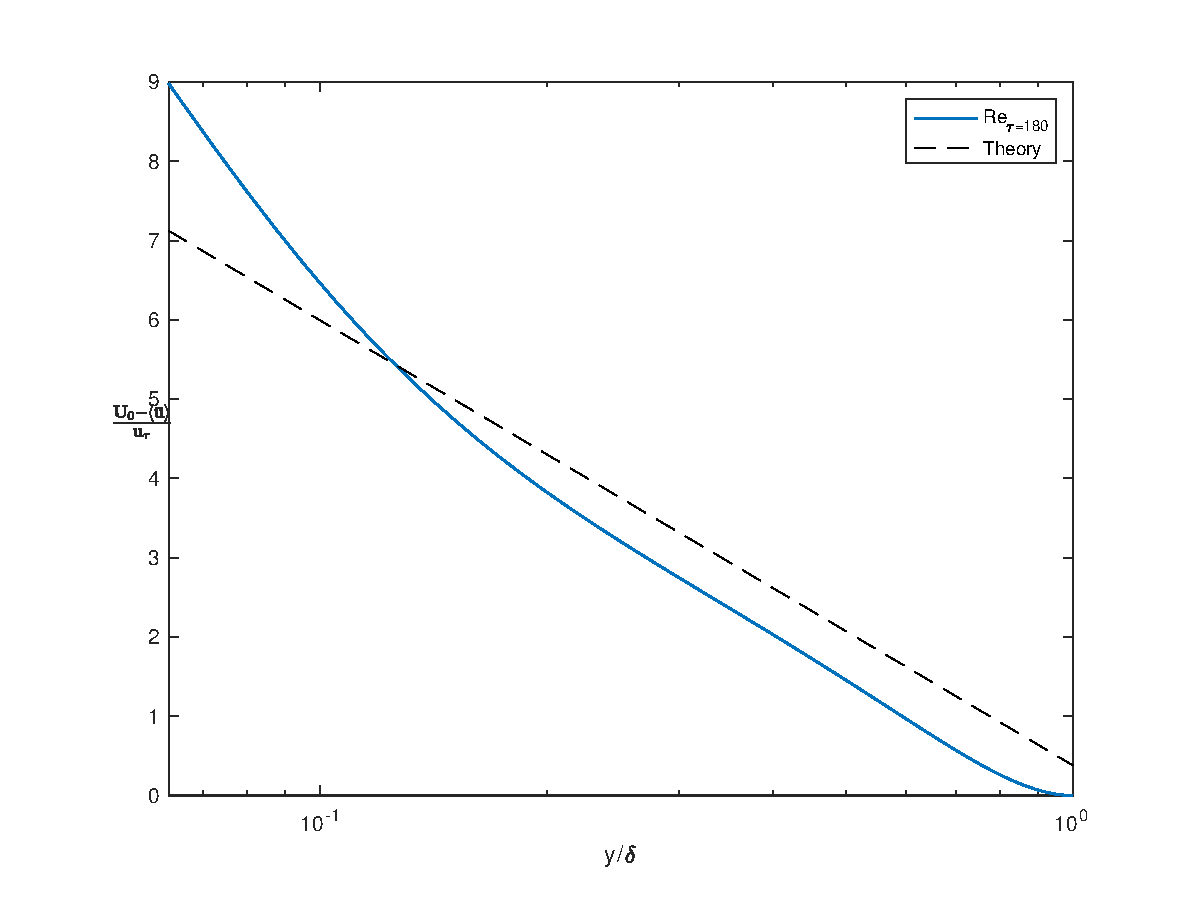
\includegraphics[scale=0.55]{grafici/velocity_defect_180.eps}
\caption{Velocity defect for a $Re_{\tau}=180$ simulation}
\label{velocity:defect:180}
\end{center} 
\end{figure}

where the constants $\kappa=0.41$ and $C^{+}\approx 5.2$, like smooth wall experiments, made by Von Karman, evidenced. \par
This velocity profile is typically denoted as \emph{the law of the wall}, and has been postulated by Prandtl in 1925.\par
Far away from the wall, the implications of the previous law originate the so called \emph{velocity defect}.
Our experimental data fits the theory, as figure~\ref{velocity:defect:180} suggest.\\~\par

The turbulence intensity trend reported on figure~\ref{rms:kmm:180} shows the comparison between the \emph{rms}, normalized by $u_{\tau}$, obtained by \emph{Kim et al.} and our results, plotted against the wall-normal distance $y^{+}$. 
The fitting is good, particularly by approaching the centerline.\par

The maxima are located between the outer region of the buffer layer and the beginning of the log-law region: the streamwise $u'/u_{\tau}$ peak is positioned at $y^{+} \approx 14$ with a value of $u'/u_{\tau} \approx 2.65$. The other two components show a smoother and less prominent behavior, with a $w'/u_{\tau} \approx 1.08$ around $y^{+} \approx 38$ and $v'/u_{\tau} \approx 0.84$ for $y^{+} \approx 50$. \\~\par

\begin{figure}
\begin{center}
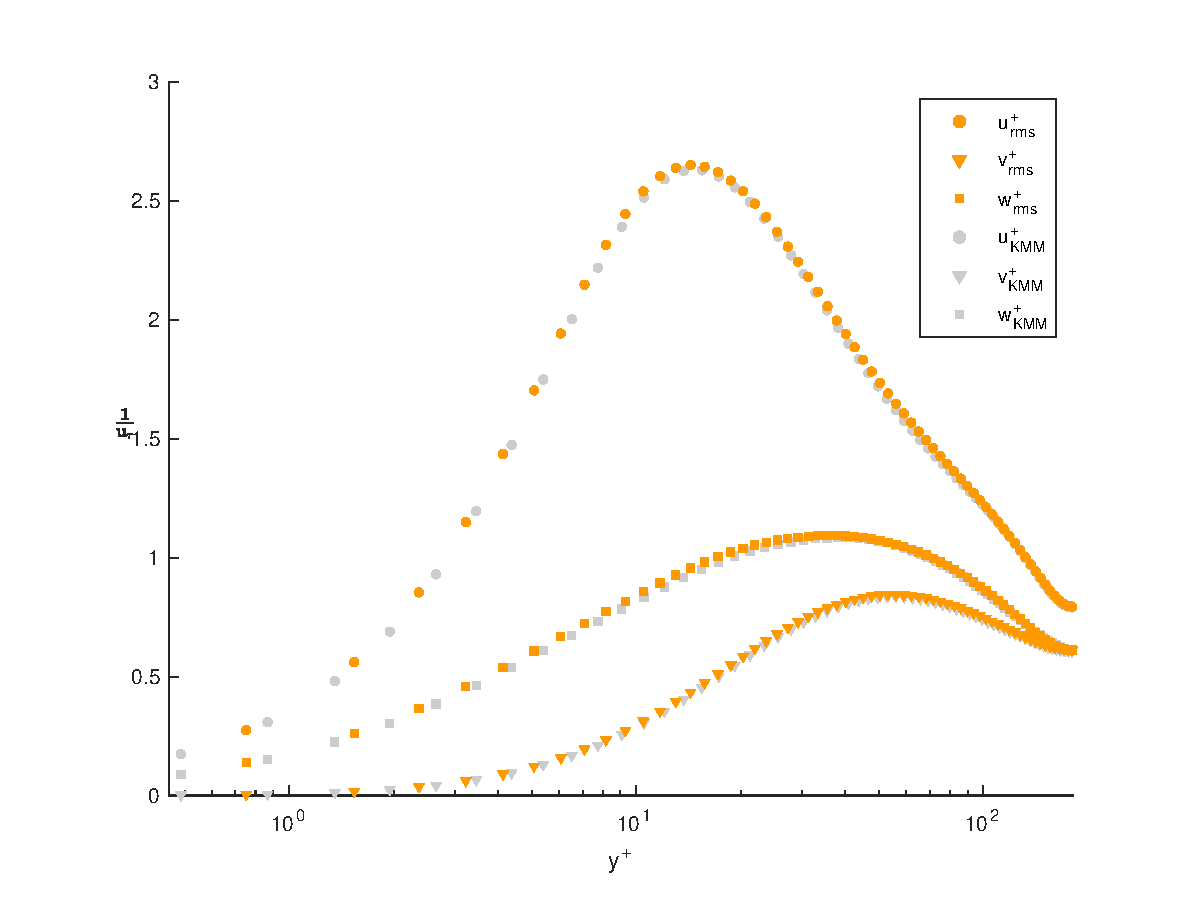
\includegraphics[scale=0.55]{grafici/rms_kmm.eps}
\caption{\emph{rms} behavior on a $Re_{\tau}=180$ simulation}
\label{rms:kmm:180}
\end{center} 
\end{figure}

A deeper knowledge of what happen close to the wall can be obtained by looking at figure~\ref{wall:rms:180}.
Such picture shows the behavior of the three \emph{rms} components, normalized by the wall coordinate, for the first 9 wall units. In dashed line it is possible to see the data from \emph{Kim et al.} \par
Once again the fitting between data is good, with both curves that follow the same trends.
It is interesting to show that for the first wall units, in the viscous sublayer, the ratio $u'/y^{+}$ remains constant, indicating constant turbulence generation. It is quite flat also the $w'/y^{+}$ behavior, while the $v'/y^{2+}$ exhibit a more slope trend.\par
The last curve is not in scale, the graph, indeed, shows a 10x magnified value, just for plotting purpose.\\~\par

\begin{figure}
\begin{center}
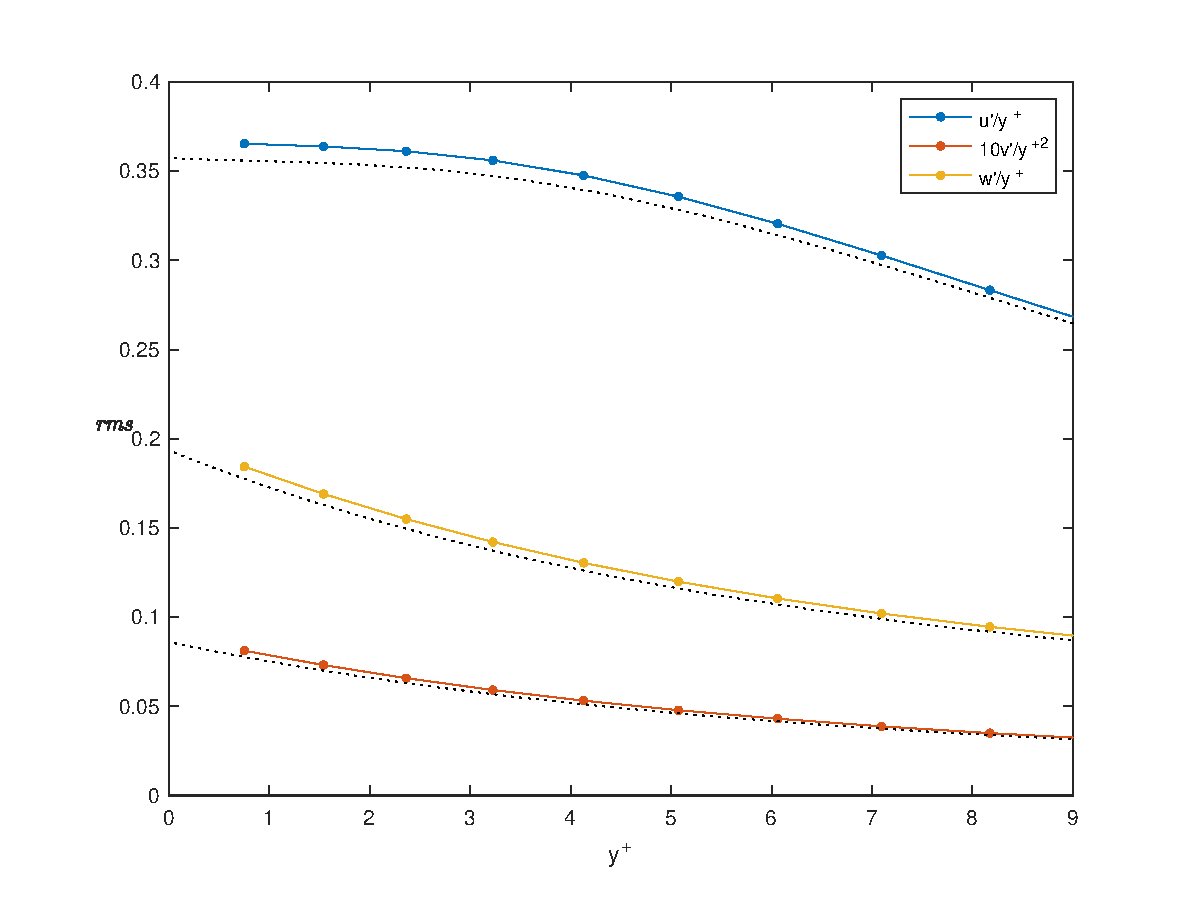
\includegraphics[scale=0.55]{grafici/wall_rms_180.eps}
\caption{Normalized \emph{rms} close to the wall for a $Re_{\tau}=180$ simulation}
\label{wall:rms:180}
\end{center} 
\end{figure}

On page~\pageref{k+budgets:180} is possible to look at the plot of the turbulent kinetic energy with the \emph{rms} terms, while figure~\ref{tke:prod:180} shows the \emph{production term}, defined as $P=-\langle u'v'\rangle \partial{\bar{u}}/\partial{y}$.\par
The two images highlight that the energy associated with the turbulence tends to develop close to the walls, and lose effectiveness once departing from there.\par
The \emph{production term} is part of the so called turbulent kinetic energy budgets and plays a key role in the interaction of the mean energy equation and TKE. The action of the mean velocity gradients working against the Reynolds stresses removes kinetic energy from the mean flow and transfers it to the fluctuating velocity field. \par
By looking at figure~\ref{tke:prod:180} we can clearly see that its contribution concentrated near the walls, with the peak around $y^{+} \approx 12$, and tends to become zero approaching the half channel height. \\~\par

\begin{figure}
\begin{center}
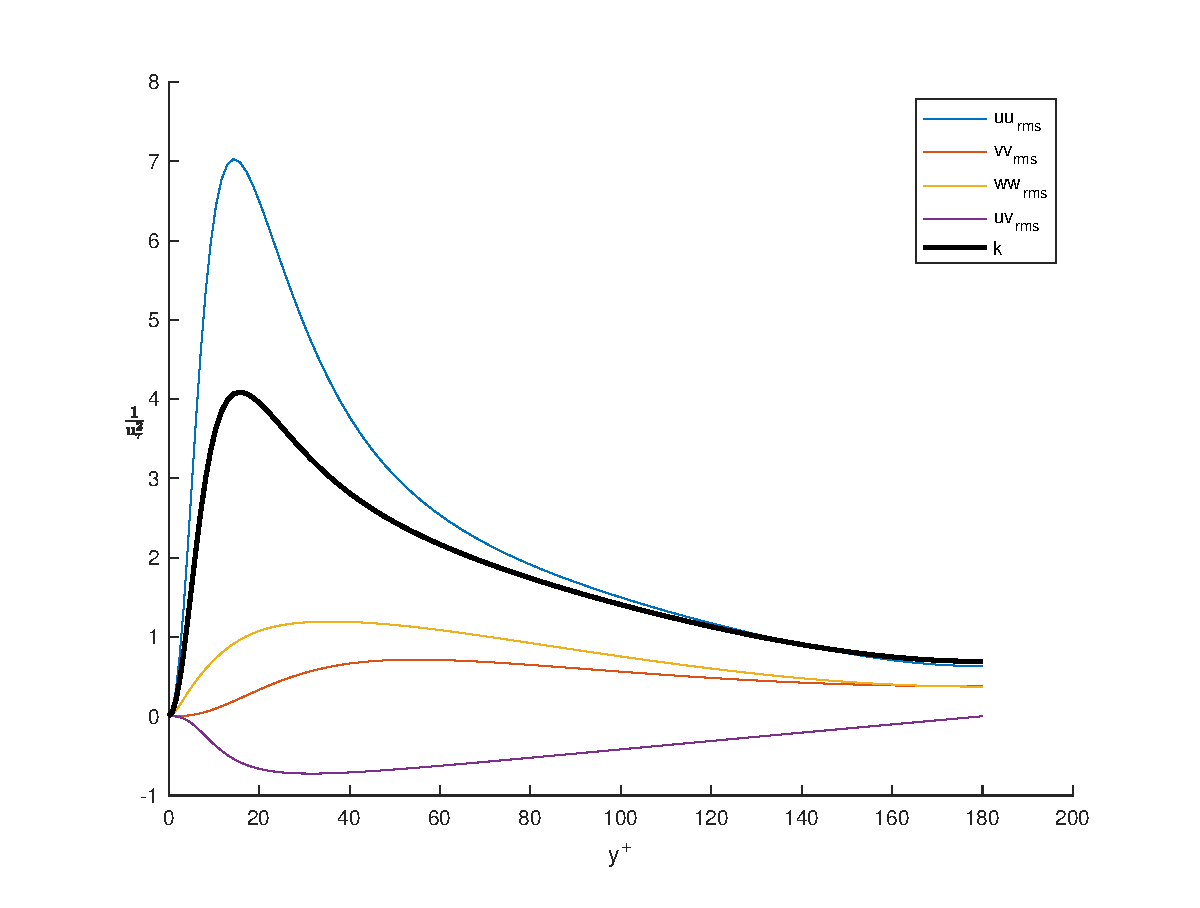
\includegraphics[scale=0.55]{grafici/budget+k_180.eps}
\caption{TKE and \emph{rms} terms for a $Re_{\tau}=180$ simulation}
\label{k+budgets:180}
\end{center} 
\end{figure}

\begin{figure}
\begin{center}
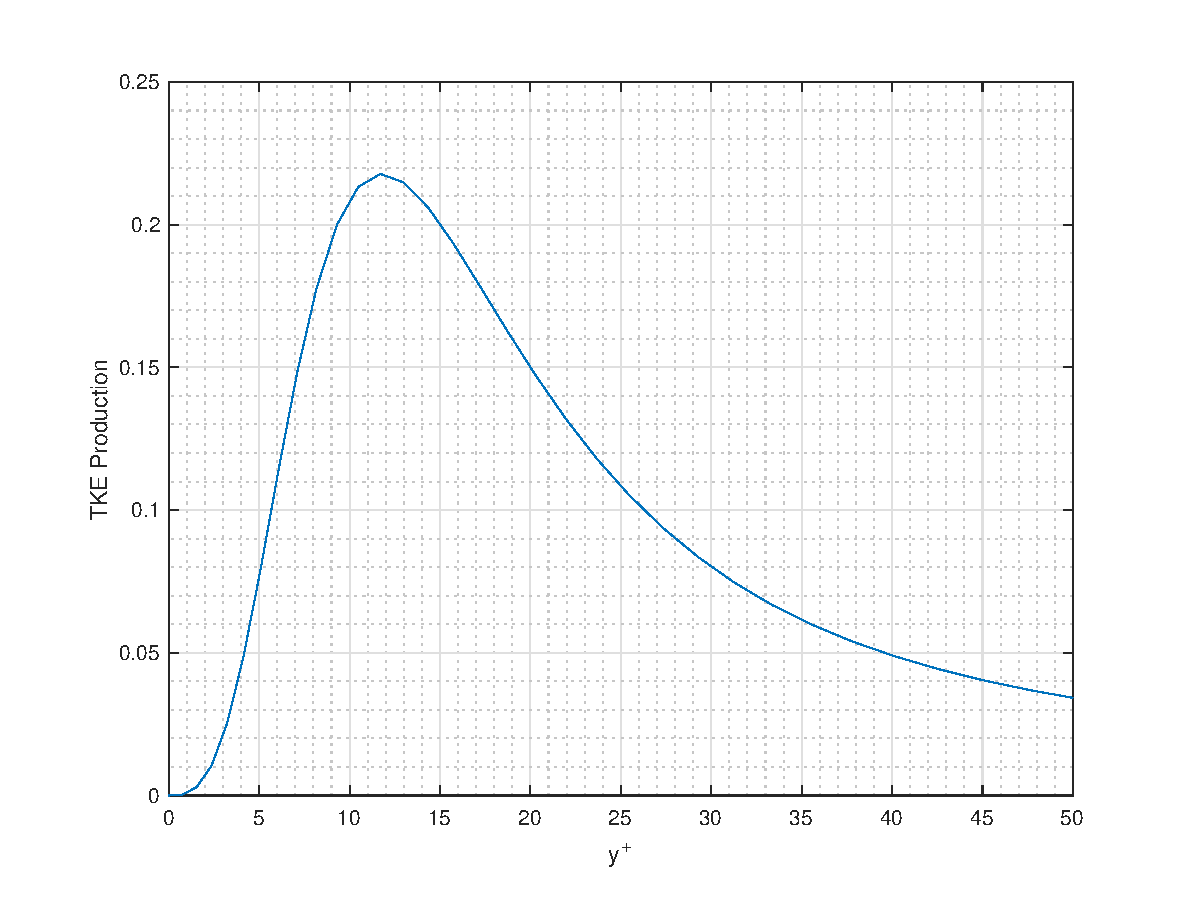
\includegraphics[scale=0.55]{grafici/tke_prod_180.eps}
\caption{Production term of the TKE eq. normalized by $Re_{\tau}=180$}
\label{tke:prod:180}
\end{center} 
\end{figure}

The \emph{production} peak occurs where the Reynolds stresses becomes equal to the viscous ones.
On figure~\ref{stresses:180} we reported the plot of the normalized total shear stress, with its contributions, in which we can see evidence of curves overlapping for $y\approx 12$.\par


\begin{figure}
\begin{center}
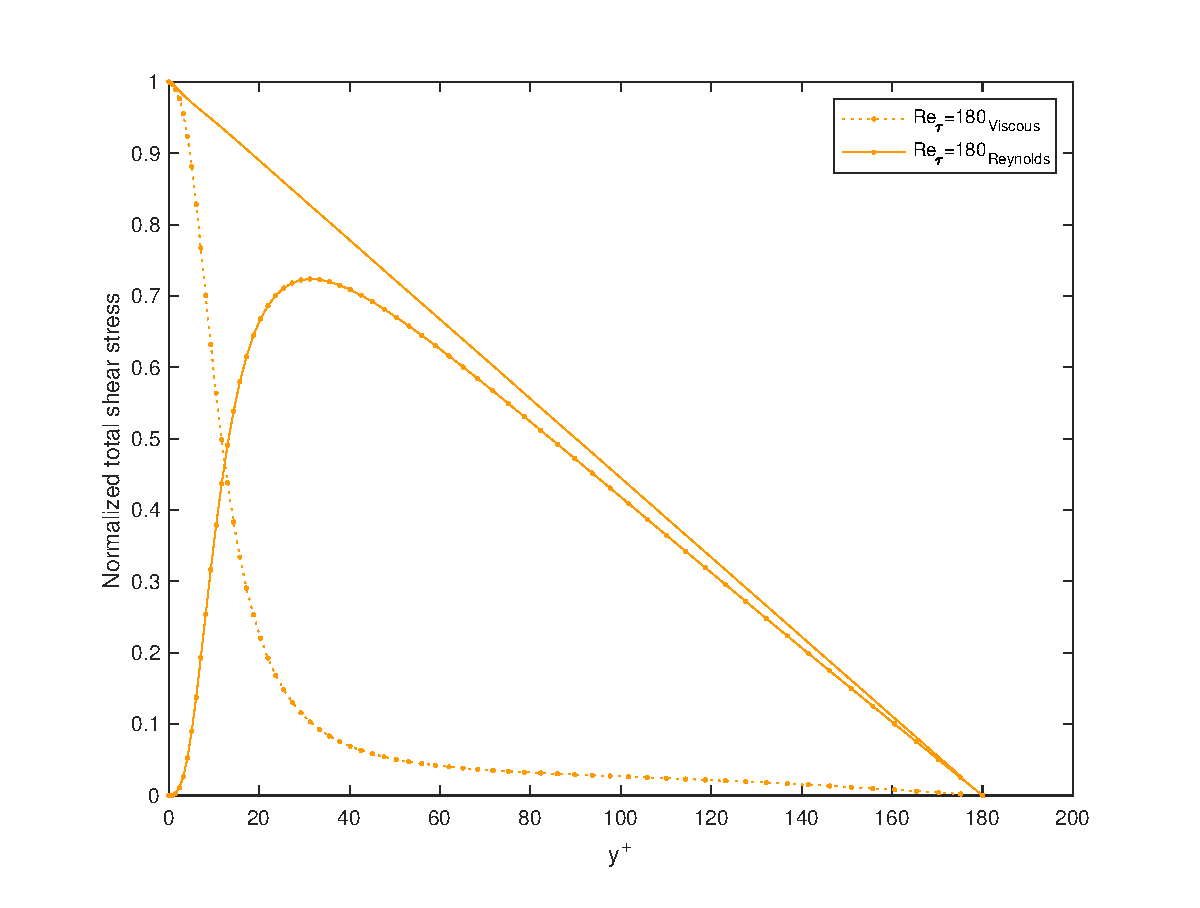
\includegraphics[scale=0.55]{grafici/stresses_180.eps}
\caption{Normalized total shear stress for a $Re_{\tau}=180$ simulation}
\label{stresses:180}
\end{center} 
\end{figure}